\documentclass[a4j,10pt,oneside,openany]{jsbook}
%
\usepackage{amsmath,amssymb}
\usepackage{bm}
\usepackage[dvipdfmx,hiresbb]{graphicx}
\usepackage{ascmac}
\usepackage{makeidx}
%
%\makeindex
%
\newcommand{\diff}{\mathrm{d}}  %微分記号
\newcommand{\divergence}{\mathrm{div}\,}  %ダイバージェンス
\newcommand{\grad}{\mathrm{grad}\,}  %グラディエント
\newcommand{\rot}{\mathrm{rot}\,}  %ローテーション
\newcommand{\btu}{\bigtriangleup} % triangle mark
\newcommand{\mr}{\mathrm}
%
\setlength{\textwidth}{\fullwidth}
\setlength{\textheight}{44\baselineskip}
\addtolength{\textheight}{\topskip}
\setlength{\voffset}{-0.6in}
%
\title{{\Huge \textbf{Dr.Hongoの数理科学ゼミ 第167問}}\\}
\author{Yuji Hiramatsu}
\date{}
%
%
%
\begin{document}
%
%
\maketitle
%\frontmatter
%\tableofcontents
%
%
%\mainmatter

%\chapter{...}
%\begin{abstract}
%...
%...
%\end{abstract}

{\Huge 167問 解答}

\vspace{3\baselineskip}


{\Large (1)}
\\
\\
題意から、
\[ f(x)=ax+\frac{1}{x} \]
\[ f'(x)=\frac{ax^2-1}{x^2} \]
であるので、$a$の値によって場合分けをする。\\
\\
(i) $a \leq 0$の時\\
$f'(x) < 0$であるので、$f(0)=+\infty$、$f(1)=1+a$より、\\
\[ \underline{f(x) \geq 1+a} \]
\\
(ii) $0 < a < 1$の時\\
$f'(x)=\frac{ax^2-1}{x^2}=0$の実数解$x=\pm \frac{1}{\sqrt{a}}$が存在する。\\
$0 < a < 1$なので、$1<\frac{1}{\sqrt{a}}$であることから、$0 < x \leq 1$においては、$f(x)$は単調減少である。よって、\\
\[ \underline{f(x) \geq 1+a} \]
\\
(iii) $1 \leq a$の時\\
$0<\frac{1}{\sqrt{a}}<1$であるので、定義域の中に極値が存在し、$f'(x)$の符号より$x=\frac{1}{\sqrt{a}}$は極小値であると分かる。\\
よって、$f(\frac{1}{\sqrt{a}})=2\sqrt{a}$から、
\[ \underline{f(x) \geq 2 \sqrt{a}} \]

\vspace{1\baselineskip}

{\Large (2)}
\\
\\
$ 0 < x $であるので、\\
\[ a x^2 - b x + 1 = 0 \Leftrightarrow ax+\frac{1}{x}=b \]
と式変形することができる。\\
(1)の答えを利用すると、\\
\\
(i) $a < 1$の時\\
\[ f(x)=ax+\frac{1}{x}=b \]
が解をもつ条件を調べればよく、$f(x) \geq 1+a$であったので、\\
\[ \underline{b \geq 1+a}\]
が、$(a,b)$の条件となる。\\
\\
(ii) $a \geq 1$の時\\
上記と同様に考えると、
\[ \underline{b \geq 2\sqrt{a}} \]
が、$(a,b)$の条件となる。\\
以上を図示すると、下図となる。


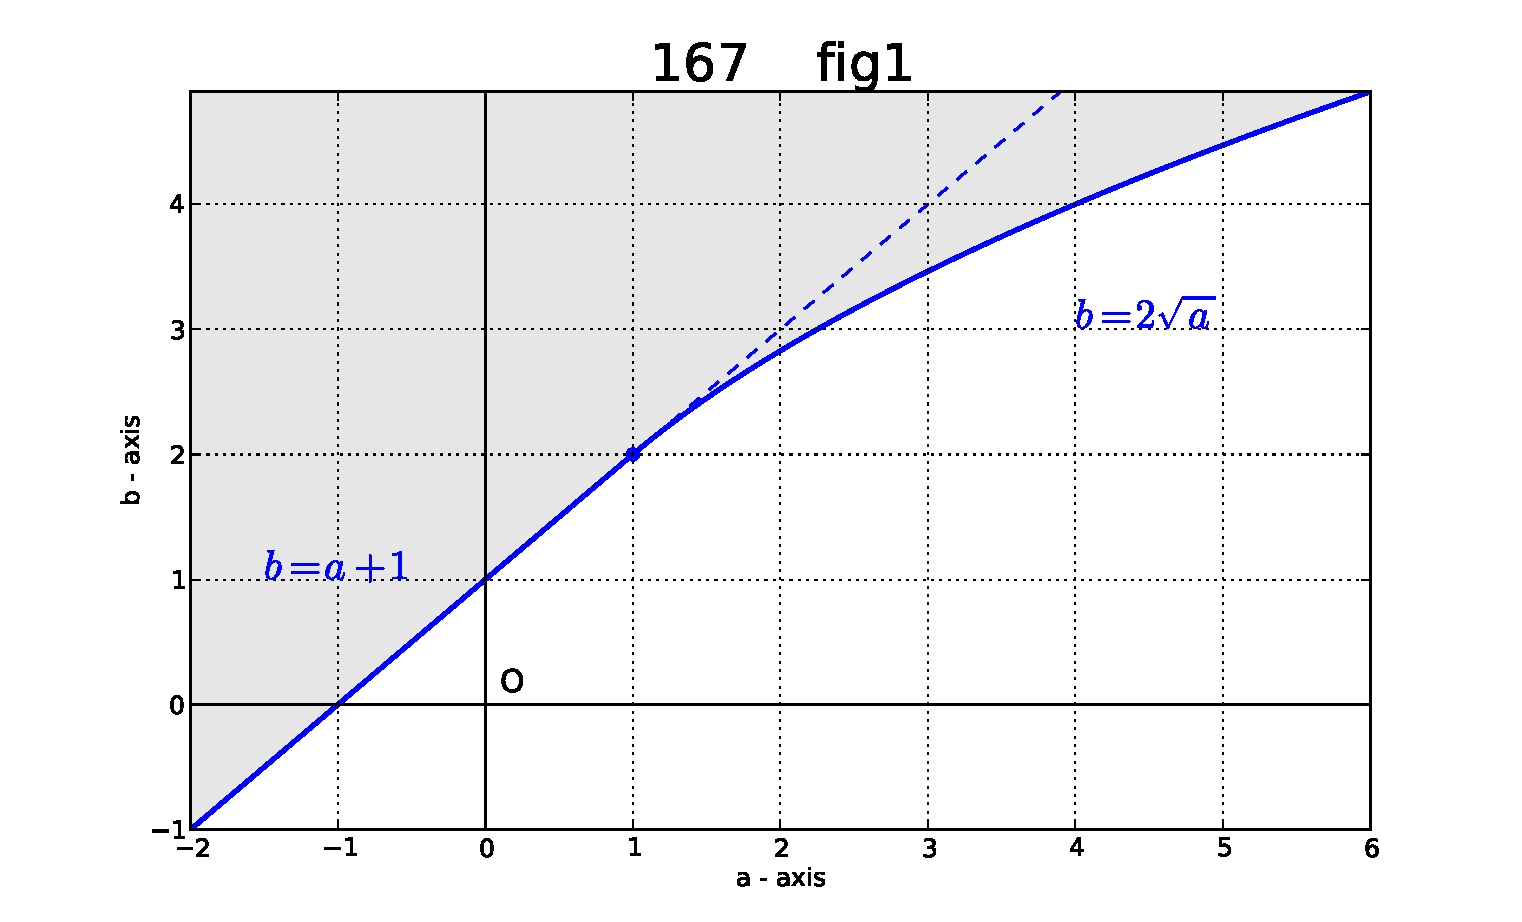
\includegraphics[width=15cm]{figure_1.pdf}


\vspace{1\baselineskip}






\end{document}











